\section{第3讲\quad 几何}

\item {
    在长方形$ABCD$中, $P,Q$分别是$AD,BC$的中点, $EM\mathop{//}NF\mathop{//}AD$, $AE=CF=6$,影部分面积为51, 那么$AD$的长度为\underline{\hbox to 20mm{}}.
    \begin{figure}[H] 
        \centering
        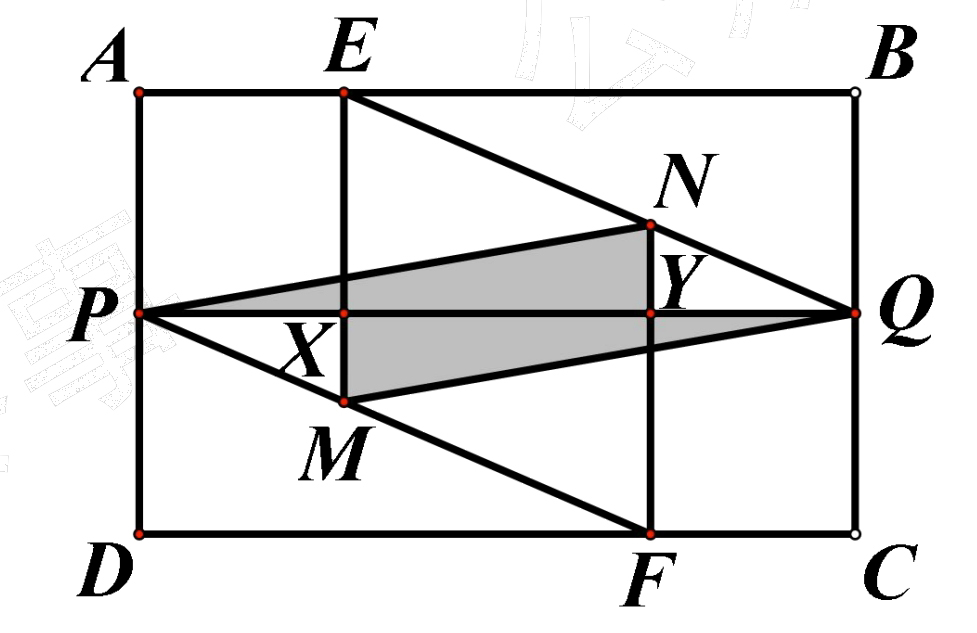
\includegraphics[width=0.4\textwidth]{./pics/Chapter_3/1.png}
    \end{figure}
    \vspace{1cm}
    % 17
}

\item {
    如图,边长为24的大正方形被分成了五个周长相等的长方形,那么阴影长方形的面积是 \underline{\hbox to 20mm{}}.
    \begin{figure}[H] 
        \centering
        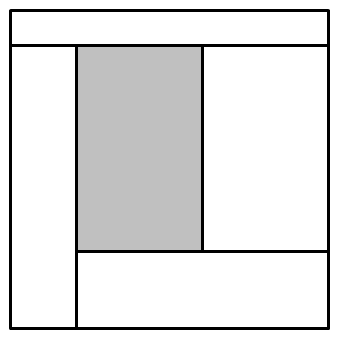
\includegraphics[width=0.2\textwidth]{./pics/Chapter_3/2.png}
    \end{figure}
    \vspace{1cm}
    % 
}

\item {
    如图,正六边形ABCDEF中,以AB为边长向内作正方形ABGH,CG与FH交于点M.\\
    (1)如果正六边形ABCDEF的边长是20,那么三角形AFH的面积是\underline{\hbox to 20mm{}}.\\
    (2)如果正六边形ABCDEF的面积是24,那么阴影部分面积之和是\underline{\hbox to 20mm{}}.
    \begin{figure}[H] 
        \centering
        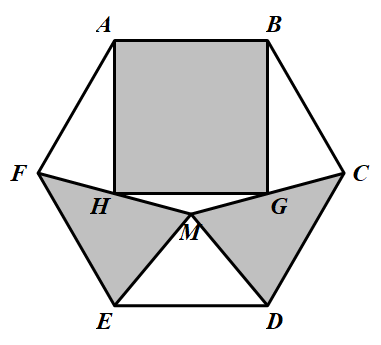
\includegraphics[width=0.4\textwidth]{./pics/Chapter_3/3.png}
    \end{figure}
    \vspace{1cm}
    % 
}
\item {
    如图,一个大正方形被分割成了周长依次为70、80、90、100的四个小长方形;那么,其中最小的小长方形的面积是\underline{\hbox to 20mm{}}.
    \begin{figure}[H] 
        \centering
        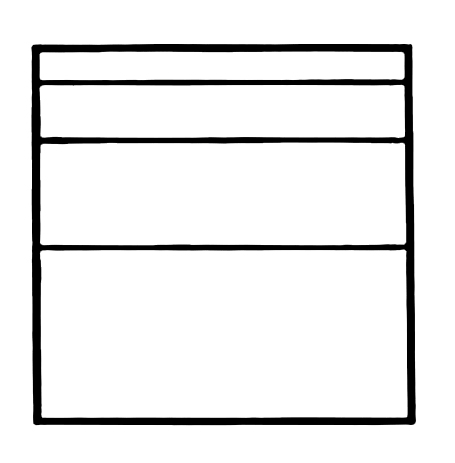
\includegraphics[width=0.2\textwidth]{./pics/Chapter_3/4.png}
    \end{figure}
    \vspace{1cm}
    % 
}

\item {
    {两个完全一样的长方形如图摆放,如果整个图形的面积是 420平方厘米,那么阴影部分的面积是\underline{\hbox to 20mm{}}平方厘米.} 
    \begin{figure}[H] 
        \centering
        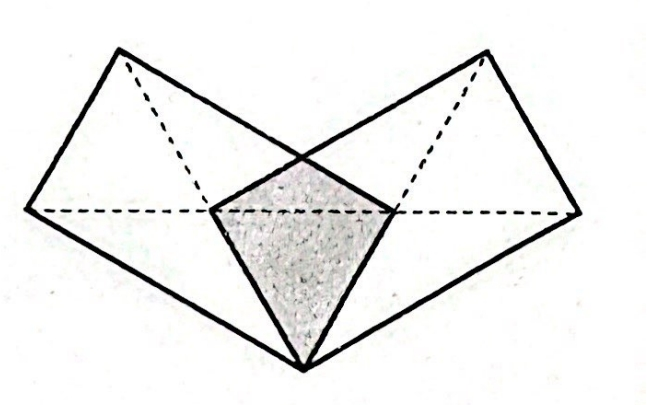
\includegraphics[width=0.4\textwidth]{./pics/Chapter_3/5.png}
    \end{figure}
    \vspace{1cm}
    % 84
}
\item {
    {在一个长方形纸片的左下角剪掉一个小长方形,
    再切成三块, 这三块恰好可以拼成一个三角形,
    若长方形的宽为12, AB的长度是CD的5倍,
    那么EC的长度为\underline{\hbox to 20mm{}}.} 
    \begin{figure}[H] 
        \centering
        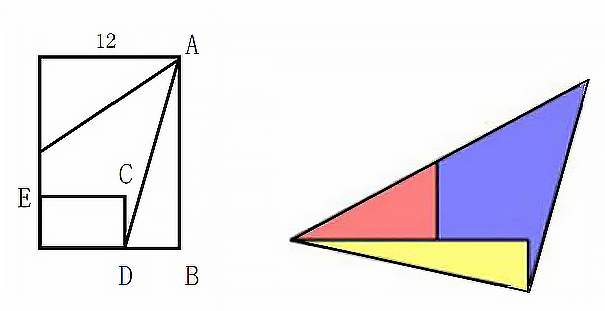
\includegraphics[width=0.6\textwidth]{./pics/Chapter_3/6.png}
    \end{figure}
    \vspace{1cm}
    % 
}

\item {
    {如图所示,一个正五边形与两个正六边形相邻,它们的边长相等。则$\angle ABC = $\underline{\hbox to 20mm{}}.} 
    \begin{figure}[H] 
        \centering
        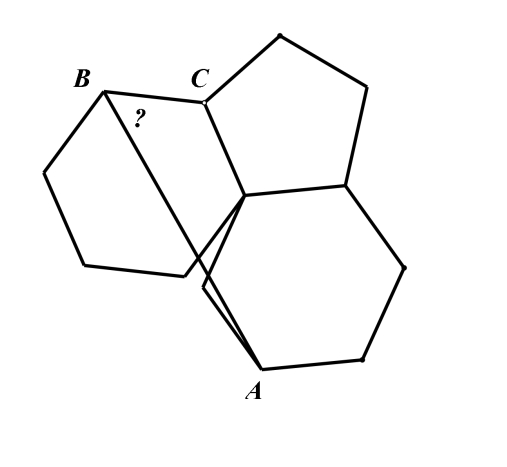
\includegraphics[width=0.4\textwidth]{./pics/Chapter_3/7.png}
    \end{figure}
    \vspace{1cm}
    % 华杯202103
}
\item {
    {如图,三角形 ABC和三角形 ADE是 $\angle A=90\degree$ 的等腰直角三角形,点 M 是 BC 的中点。已知$AB=AC=DF=FM=EG=GM$, $\angle FDE = \angle GED=9\degree$ 且点F和点G在三角形ADE以外. 问$\angle FMG$ 的度数是( )度.} 
    \begin{figure}[H] 
        \centering
        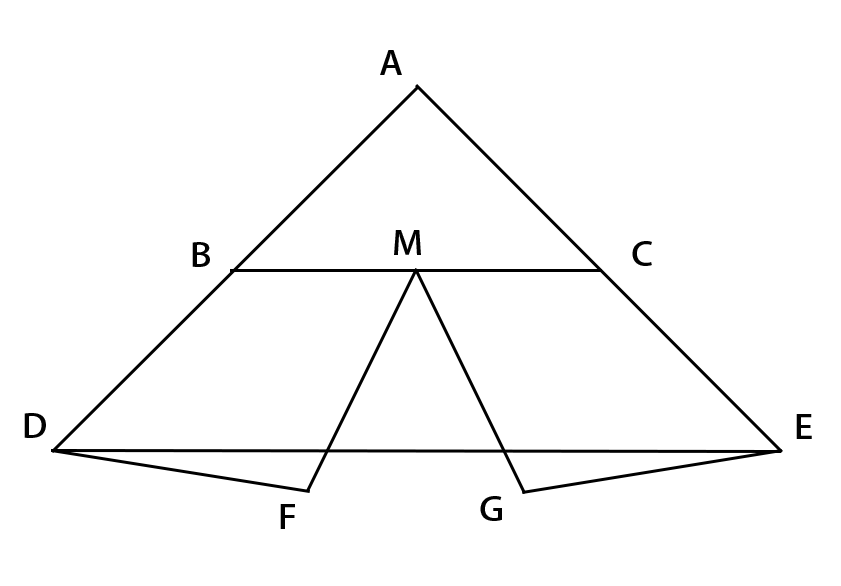
\includegraphics[width=0.4\textwidth]{./pics/Chapter_3/8.png}
    \end{figure}
    \vspace{1cm}
    % 华数真题2021-2023(小中组).pdf, 2022.2.19线上小中组解析1.pdf; 54
}

\item {
    {在下图中,$\angle 1 + \angle 2 + \angle 3 + \angle 4 - \angle 5=$ \underline{\hbox to 20mm{}} $\degree$.} 
    \begin{figure}[H] 
        \centering
        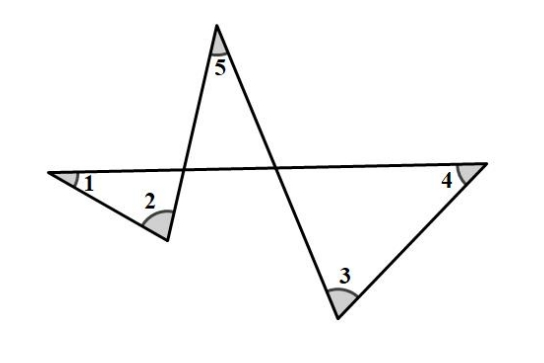
\includegraphics[width=0.4\textwidth]{./pics/Chapter_3/9.png}
    \end{figure}
    \vspace{1cm}
    % 华数真题2021-2023(小中组).pdf
}
\item {
    {如图所示,一个正方形纸片ABCD沿对角线BD剪成两个三角形.第一步操作,将三角形ABD竖直向下平移3厘米至三角形EFG;第二步操作,将三角形EFG竖直向下再平移5厘米至三角形HIJ.第一步操作后两张纸片重叠的面积与第二步操作后两张纸片重叠的面积相等,那么这个正方形纸片ABCD的面积是 \underline{\hbox to 10mm{}} 平方厘米.} 
    \begin{figure}[H] 
        \centering
        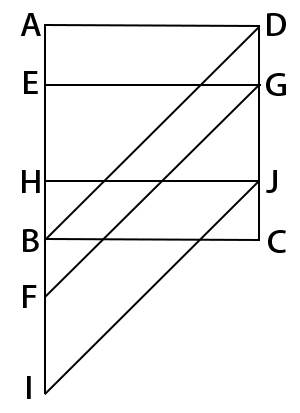
\includegraphics[width=0.2\textwidth]{./pics/Chapter_3/10.png}
    \end{figure}
    \vspace{1cm}
    % 2018年第二十三届“华罗庚金杯”少年数学邀请赛初赛试卷(小中组).doc; 121
}

\item {
    {从四边形4个内角取2个求和,共有6个和数,则大于180°的和最多有 \underline{\hbox to 20mm{}} 个.} 
    \begin{figure}[H] 
        \centering
        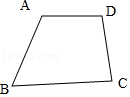
\includegraphics[width=0.2\textwidth]{./pics/Chapter_3/11.png}
    \end{figure}
    \vspace{1cm}
    % 华杯2018; 3
}
\item {
    {如图,将一个正方形硬纸片的四个角分别剪去一个等腰直角三角形,最后剩下一个长方形.正方形边长和三角形直角边长都是整数.若剪去部分的总面积为40平方厘米,则长方形的面积是 \underline{\hbox to 20mm{}} 平方厘米.} 
    \begin{figure}[H] 
        \centering
        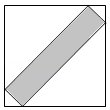
\includegraphics[width=0.2\textwidth]{./pics/Chapter_3/12.png}
    \end{figure}
    \vspace{1cm}
    % 2017年第二十二届“华罗庚金杯”少年数学邀请赛决赛试卷(小中组).doc; 24
}

\item {
    {如图所示,两个边长为6的正方形ABFE和CDEF拼成长方形ABCD.G为DE的中点.连接BG交EF于H.求图中五边形CDGHF的面积.} 
    \begin{figure}[H] 
        \centering
        
\includegraphics[width=0.4\textwidth]{./pics/Chapter_3/13.png}
    \end{figure}
    \vspace{1cm}
    % 华杯2017; 33
}
\item {
    {图中的八边形是将大长方形纸片剪去一个小长方形得到.则至少需要知道(\quad)条线段的长度,才可以计算出这个八边形的周长.} \\
    {A. 4\quad B. 3\quad C. 5\quad D. 10}
    \begin{figure}[H] 
        \centering
        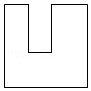
\includegraphics[width=0.2\textwidth]{./pics/Chapter_3/14.png}
    \end{figure}
    \vspace{1cm}
    % 2017年第二十二届“华罗庚金杯”少年数学邀请赛初赛试卷(小中组).doc; B
}

\item {
    {如图,在两张大小相同的大长方形纸片上,分别在角和边上各剪下一个大小相同的小正方形.若图\textcircled{2}阴影部分的周长比图\textcircled{1}阴影部分的周长多17厘米,那么剪下的小正方形周长为 \underline{\hbox to 10mm{}} 厘米.} \\
    \begin{figure}[H] 
        \centering
        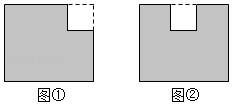
\includegraphics[width=0.4\textwidth]{./pics/Chapter_3/15.png}
    \end{figure}
    \vspace{1cm}
    % 华杯2017; 34
}
